% class
\documentclass[a4paper,12pt,xelatex,ja=standard]{bxjsarticle}

% packages
%% mathematical notations
\usepackage{amsthm,amsmath,amssymb,amsfonts} % mathematical notations
\usepackage{bm} % bold character
\usepackage{latexsym} % more mathematical notations
\usepackage{physics} % physical notations
%% graphs
\usepackage{graphicx, xcolor} % graph
\usepackage{circuitikz} % for circuit elements
\usepackage{float} % positioning of graphs
\usepackage{siunitx} % SI units
\usepackage{tikz} % graphic elements
\usepackage{wrapfig} % must be after float package.
\usepackage{askmaps} % Karnaugh map
%% type system
\usepackage{bussproofs} % proof tree
%% code
\usepackage[ruled,vlined]{algorithm2e} % pseudo code
\usepackage{listings} % source code
\usepackage{inconsolata}
\lstset{
  basicstyle=\footnotesize,
  numbers=left,
  frame={tb}
}
\usetikzlibrary{automata, positioning}
\tikzset{
  ->,
  >={Stealth[round]},
  auto,
  every state/.style={draw}
}

% Basic information
\title{電子情報学専攻 \, 専門 \\ 平成26年 \, 解答・解説}
\author{diohabara}
\date{\today}

\begin{document}
\maketitle

\section*{第1問\ 電気・電子回路}

\section*{第2問\ 計算機アーキテクチャ}
\subsection*{(1)}
\subsubsection*{$\alpha$}

\subsubsection*{$\beta$}

\subsubsection*{$\gamma$}

\subsubsection*{$\delta$}

\subsection*{(2)}
\subsubsection*{(i)}
\subsubsection*{(ii)}

\subsection*{(3)}

\subsection*{(4)}

\subsection*{(5)}

\section*{第3問\ アルゴリズムとデータ構造}
\subsection*{(1)}
各ステップにおいて、$B$に含まれる頂点と$V \setminus B$に含まれる頂点を結ぶ辺のうち重みが最小である辺$e = \{u, v\} (u \in V \setminus, v \in B)$が最小全域木に含まれることを示す。\\
連結グラフなら最小全域木が必ず存在し、このうちの1つを$T \subseteq E$とする。$T$が$e$を含むならok。
含まない場合は、$B$と$V \setminus B$を結ぶある辺$f = e$存在し、$(f\text{の重み}) \geq (e\text{の重み})$が成立する。
この最小全域木には$u, v$をつなぐパス($f$を含む)が存在するので、$T$に$e$を追加すると閉路ができ、そこから$f$を取り除いた辺集合は全域木であることが言える。
重みの総和は$T$の重みの総和以下であるのでこれもまた最小全域木である。

\subsection*{(2)}
最小全域木は以下の通り。
\begin{figure}[H]
  \centering
  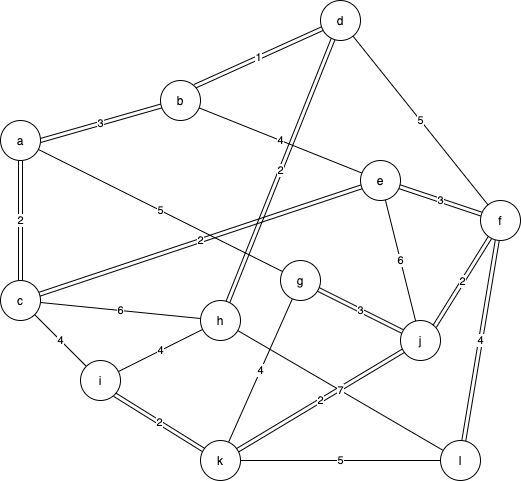
\includegraphics[width=11cm]{images/2016_min_spanning_tree.png}
\end{figure}

\subsection*{(3)}
\begin{lstlisting}[language=Python, caption=プリム法]
def primMST():
    T = set()
    for i in range(1, n):
        edge = set()
        min_cost = inf
        for v in (V - B):
            u = nearest[v]
            if mindist[v] == -1:
                continue
            if L[u, v] < min_cost:
                min_cost = L[u, v]
                edge = {u, v}
        T.append(edge)

\end{lstlisting}

\subsection*{(4)}
$O(|V|^2)$\\
nearestとmindistの更新を素朴にやると$O(|V|^2)$なので、全体で$O(|V|^2)$だが、$V \setminus B$に含まれる各頂点までの最小コストを記録しておいて、各ステップにおいてその最小コストが最小の頂点を$V$に加えるようにすれば$O(|V|^2)$に計算量をできる。

\subsection*{(5)}
二分ヒープとは二分木を使って実装されるヒープのことである。
ヒープとは各ノードはその子ノードよりも大きいか等しい。また、平衡二分木となっている。

\subsection*{(6)}
\subsubsection*{適用の仕方}
二分ヒープheapに$B$に含まれる頂点から伸びている辺を入れて重みが小さい順に取り出すことにする。\\
各ステップにおいて
\begin{enumerate}
  \item heapから辺を1つ取り出す
  \item その辺の両端点がそれぞれ$B$と$V \setminus B$に含まれていればその辺を採用して新たに$V$に加わった頂点から伸びている辺をすべてheapに追加する。そうでなければその辺は削除して1に戻る
\end{enumerate}
という処理を行う。

\subsubsection*{計算量}
heapへの追加・削除はそれぞれ$O(\log |E|)$でできて、各頂点から伸びる辺の探索は$O(|V|)$なので全体で$O(|V|^2 \log |E|)$。
これでは(4)で見積もった計算量より悪い。しかし、グラフを隣接リストで実装すると全体で$O((|V| + |E|) \log |E|) = O(|E| \log |E|)$となる。

\subsubsection*{頂点の数$n$と辺の数$m$の関係}
完全グラフのような辺の数$m$が頂点の数$n$の事情のオーダーの場合は計算量が悪化するが、そこまで辺が大きくなければ効率化できる。

\section*{第4問\ 情報理論}
\subsection*{(1)}

\subsection*{(2)}

\subsection*{(3)}

\subsection*{(4)}

\subsection*{(5)}

\subsection*{(6)}

\section*{第5問\ 信号処理}
\subsection*{(1)}

\subsection*{(2)}

\subsection*{(3)}

\subsection*{(4)}

\end{document}

